%        File: DesignDocument.tex
%     Created: 一 3月 26 01:00 下午 2018 C
% Last Change: 一 3月 26 01:00 下午 2018 C
%
\documentclass[UTF8,noindent]{ctexart}
\usepackage[a4paper,left=2.0cm,right=2.0cm,top=2.0cm,bottom=2.0cm]{geometry}
\usepackage{hyperref}
\usepackage{url}
\usepackage{graphicx}
\usepackage{amsmath}
\usepackage{amssymb}
\usepackage{enumitem}
\usepackage{tikz}
\usepackage{float}
\usepackage{xeCJK}
\usepackage{listings}
\usepackage{xcolor}
\lstset{language = c++,numbers=left, showstringspaces=false,keywordstyle= \color{ blue!70 },commentstyle=\color{red!50!green!50!blue!50}, frame=shadowbox, rulesepcolor= \color{ red!20!green!20!blue!20 } 
} 
\CTEXsetup[format={\Large\bfseries}]{section}
\usetikzlibrary{graphs}
%\newtheorem*{lemma}{Lemma}
\title{\CJKfamily{zhkai}计算机网络研讨课实验报告}
\author{{\CJKfamily{zhkai}冯吕}\ $2015K8009929049$}
\date{\today}
\begin{document}
\maketitle
\zihao{5}
\CJKfamily{zhsong}
%\begin{center}
%  \begin{tabular}{|p{15cm}|}
%    \hline
\section*{{\CJKfamily{zhhei}实验题目}}高效$IP$路由查找实验
%\hline
\section*{{\CJKfamily{zhhei}实验内容}}
本次实验需要实现路由查找中的$IP$最长前缀查找。

实验内容分为两部分:
\begin{itemize}
  \item 实现最基本的单比特匹配的前缀树查找;
	\item 实现多比特的前缀树查找以及优化:叶推、压缩向量以及压缩指针。
\end{itemize}

然后,基于数据集$forwarding-table.txt$,来进行测试,并比对两种不同方法的性能开销。
\section*{{\CJKfamily{zhhei}实验流程}}
\subsection*{单比特前缀树}
在本次实验中,首先要实现最基本的前缀树查找,实现该查找的类定义如下:
\begin{lstlisting}
class PTree{
	public :
		u32 SubNet;
		u8 PreLen;
		u8 Port;
		PTree(){
			SubNet = 0;
			PreLen = 0;
			Port = 0;
			Child[0] = Child[1] = NULL;
		};
		u32 StrToIp(const char *s);
		virtual bool ConstructTree();
		bool Insert(PTree *Node);
		bool Pleafpush(PTree *Node);
		PTree *Search(u32 IP);
		virtual bool DestructTree();
		virtual ~PTree(){
		};
		void dumpNode();
	private :
		PTree *Child[2];
};
\end{lstlisting}

在该类的成员中,$SubNet$存储子网,$PreLen$存储前缀长,$Port$存储对应的端口,以及两个指向子树的指针数组。构建树时将子网转换成一个$32$位无符号整数。因此,定义了一个将$str$转化为$32$位无符号数的方法。构建树时,将数据集中的每一条记录依次插入到树中,构建树的过程实际上也是一个查找的过程。查找时,则将查找$IP$和前缀树进行前缀匹配搜索。

$dumpNode$方法将查找结果以可读形式输出到标准输出。另外,当程序退出前,需要将前缀树释放($DestructTree()$)。

\subsection*{多比特前缀树}
多比特前缀树的定义如下:
\begin{lstlisting}
class MulPTree : public PTree{
	public :
		MulPTree *mChild[4];
		MulPTree(){
			SubNet = 0;
			PreLen = 0;
			Port = 0;
			mChild[0] = mChild[1] = mChild[2] = mChild[3] = NULL;
		};
		virtual bool ConstructTree();
		bool Insert(MulPTree *Node);
		MulPTree *Search(u32 IP);
		bool MleafPush(MulPTree *Node);
		bool Equal(PTree *Node){
			return Node->SubNet == SubNet
			&& Node->PreLen == PreLen 
			&& Node->Port == Port;
		}
		bool Equal(Leaf *leaf){
			return SubNet == leaf->SubNet 
			&& PreLen == leaf->PreLen
			&& Port == leaf->Port;
		};
		virtual bool isLeaf(){
			return !mChild[0] && !mChild[1] && !mChild[2] 
			&& !mChild[3];
		}
		virtual bool DestructTree();
		virtual ~MulPTree(){
		};
};
\end{lstlisting}

多比特前缀树继承单比特前缀树,它的构建和查找方法和前者基本一样。它的指向子树的指针数组大小变为$4$,另外,增加了判断两个判断查找结果是否相等的方法。

\subsection*{叶推}

叶推时,需要把所有的包含匹配前缀的中间节点下推到叶子节点。通过递归能够很方便的实现。

下面是多比特前缀树的叶推方法,单比特类似:
\begin{lstlisting}
bool MulPTree::MleafPush(MulPTree *Node){
	if (mChild[0] == NULL && mChild[1] == NULL
	&& mChild[2] == NULL && mChild[3] == NULL){
		return true;
	}
	if (SubNet != 0){
		Node->SubNet = SubNet;
		Node->Port = Port;
		Node->PreLen = PreLen;
	}
	if (mChild[0]&&mChild[1]&&mChild[2]&&mChild[3]){
		for (u8 i = 0; i != 4; ++i){
			mChild[i]->MleafPush(Node);
		}
	}
	else {
		MulPTree *NewNode = new MulPTree();
		NewNode->SubNet = Node->SubNet;
		NewNode->PreLen = Node->PreLen;
		NewNode->Port = Node->Port;
		for (u8 i = 0; i != 4; ++i){
			if (mChild[i] == NULL)
			  mChild[i] = Node;
			else 
			  mChild[i]->MleafPush(NewNode);
		}
	}
	return true;
}
\end{lstlisting}

\subsection*{压缩指针和压缩向量}
压缩指针和压缩向量是在叶推的基础上实现的,叶推之后,除了叶子节点之外,所有的中间节点的指向孩子的指针均不为空,因此,可以把中间节点和叶子节点分开,中间节点存储子孩子的标记:是叶子还是子树,以及两个指向叶子向量和子树向量的指针,而叶子节点只需要存储数据即可。

下面是中间节点的定义。
\begin{lstlisting}
class CVTree{
	public :
		bool NotLeaf[4];
		Leaf *LeafVec;
		CVTree *ChildVec;
		CVTree(){
			NotLeaf[0]=NotLeaf[1]=NotLeaf[2]=NotLeaf[3]=0;
			LeafVec = NULL;
			ChildVec = NULL;
		}
		bool ConstructCVTree(MulPTree *Tree);
		Leaf *Search(u32 IP);
		u8 Count(u8 loc);
		bool DestructCVTree();
		virtual ~CVTree(){
			if (LeafVec){
				delete[] LeafVec;
			}
		};
};
\end{lstlisting}

$ConstructCVTree$方法构建压缩指针和向量后的树,它通过前序遍历一棵完成叶推后的前缀树来进行构建,压缩指针和压缩向量可以同时实现:
\begin{lstlisting}
bool CVTree::ConstructCVTree(MulPTree *Tree){
	u8 haveChild = 0;
	u8 haveLeaf = 0;
	for(u8 i = 0; i != 4; ++i){
		if (Tree->mChild[i] && !Tree->mChild[i]->isLeaf()){
			NotLeaf[i] = true;
			++haveChild;
		}
		if (Tree->mChild[i] && Tree->mChild[i]->isLeaf()){
			++haveLeaf;
		}
	}
	if (haveLeaf + haveChild != 4){
		return false;
	}
	if (haveLeaf){
		LeafVec = new Leaf[haveLeaf];
		for (u8 i = 0, j = 0; i != 4 && j != haveLeaf; ++i){
			if (Tree->mChild[i]&& Tree->mChild[i]->isLeaf()){
				LeafVec[j].SubNet = Tree->mChild[i]->SubNet;
				LeafVec[j].PreLen = Tree->mChild[i]->PreLen;
				LeafVec[j].Port = Tree->mChild[i]->Port;
				++j;
			}
		}
	}
	if (haveChild){
		ChildVec = new CVTree[haveChild];
		for (u8 i = 0, j = 0; i != 4 && j != haveChild; ++i){
			if (Tree->mChild[i] && !Tree->mChild[i]->isLeaf()){
				ChildVec[j].ConstructCVTree(Tree->mChild[i]);
				++j;
			}
		}
	}
	return true;
}
\end{lstlisting}
\section*{{\CJKfamily{zhhei}实验结果}}
该程序运行时,输入为以点分隔的合法$IP$,由于没有对输入的合法性进入检查,因此,如果输入不合法会导致程序$crash$。
\begin{figure}[H]
  \centering
  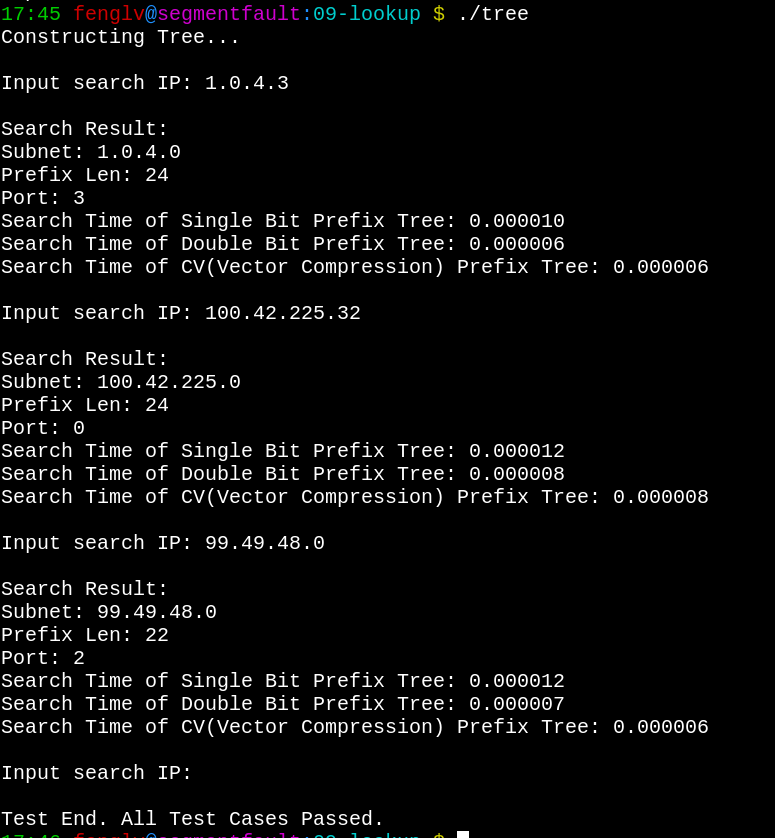
\includegraphics[scale = 0.5]{1.png}
  \caption{$IP$查找}
\end{figure}

从性能上来看,单比特的查找时间大概是双比特的两倍,因为查找过程中需要访问的节点是它的两倍。

\section*{{\CJKfamily{zhhei}结果分析}}
本次实验原本以为会比较容易,但最后实现起来发现遇到了很多的$bug$,调试时间远远超过写代码的时间,最后还导致作业没有能够按时提交实验,不过说到底还是自己的代码功底需要提升。
\end{document}


